\documentclass[12pt, letterpaper]{article}
\def\blank{\medskip\hrule\medskip}
\usepackage[T2A]{fontenc}
\usepackage[utf8x]{inputenc}
\usepackage[english, russian]{babel}
\usepackage{amsthm}
\usepackage{amssymb}
\usepackage{graphicx} 
\usepackage{wrapfig}
\usepackage{amsmath}
\usepackage[unicode, pdftex]{hyperref}

\renewcommand\qedsymbol{$\blacksquare$}
\renewcommand{\arraystretch}{2} %
\everymath{\displaystyle}

\newtheorem{theorem}{Теорема}[section]
\newtheorem{prop}{Утверждение}[section]

\usepackage[%
    left=0.50in,%
    right=0.50in,%
    top=0.50in,%
    bottom=0.50in,%
    paperheight=11in,%
    paperwidth=8.5in%
]{geometry}%

\begin{document}

\section{Ряд Лорана}
\begin{prop} Существуют $r, R \in [0, +\infty)$ такие, что $\forall z: r < |z| < R$ некоторый ряд Лорана абсолютно сходится, а также $\forall z : |z|>R$ или $|z|<r$ этот ряд расходится.
\end{prop}
\begin{proof}
Нужно воспользоваться теоремой для радиуса сходимости степенных рядов. 
\end{proof}
\begin{prop}
В кольце, лежащем строго внутри кольца сходимости, сходимость равномерная и можно дифференцировать почленно.
\end{prop}
\begin{proof}
Отсылка к свойствам степенных рядов
\end{proof}
\begin{prop}
Если голоморфная $f$ раскладывается в кольце $r < |z| < R$ в ряд Лорана, то его коэффициенты определяются однозначно и $a_n = \frac1{2\pi i} \int_{\rho \mathbb{T}} \frac{f(\xi)}{\xi^{n+1}} d\xi$, где $r < \rho < R$. 
\end{prop}
\begin{proof}
Честно проинтегрируйте то, что написано в условии и получите нужную формулу. Не забудьте, что если ряд сходится в некоторой области равномерно, то в ней можно интегрировать почленно.
\end{proof}
\begin{theorem}[Теорема Лорана]
$f \in H(r < |z| < R)$. Тогда $f$ раскладывается в этом кольце в ряд Лорана.
\end{theorem}
\begin{proof}
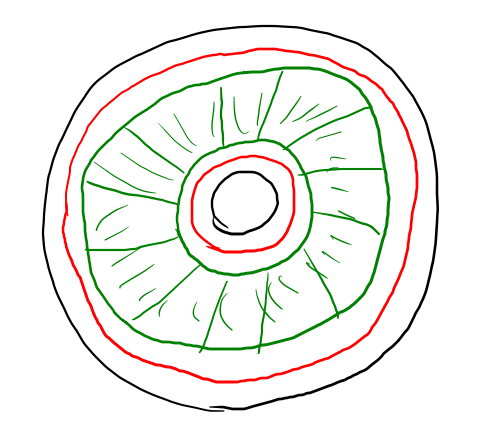
\includegraphics[scale=0.6]{1.png}\\
Возьмите $r < r_1 < r_2 < R_2 < R_1 < R$. Раскладывать в ряд Лорана будем для $r_2 \leq |z| \leq R_2$. Для этого напишем для них интегральную формулу Коши по компакту. Далее стандартным образом раскидаем всё на ряды с помощью геометрической прогрессии. Не забываем про то, почему можно менять сумму с интегралом: тут работает признак Вейрштрасса: ряды будут равномерно сходиться.
\end{proof}
\begin{prop}
Неравенство Коши: $|a_n| \leq \frac{M_r}{r^n}$. 
\end{prop}
\begin{proof}
Оцените интеграл самым простым образом.
\end{proof}
\begin{prop}
$f \in H(r < |z| < R)$. Тогда существует $g \in H(R\mathbb{D})$ и $h \in H(\mathbb{C} \setminus r\mathbb{D})$, такие что $f = g + h$. Если добавить условие $\lim_{z \rightarrow \infty} h(z) = 0$, то такое разложение единственно.
\end{prop}
\begin{proof}
В качестве $g$ надо взять правильную часть ряда Лорана, в качестве $h$ -- главную часть. \\
Единственность. Пусть $f = g_1 + h_1 = g_2 + h_2$. \\
$F(z) = g(z)-g_1(z)$ при $|z| < R$ и $h_1(z) - h(z)$ при $|z| > r$. Если $r < |z| < R$, то неважно какую мы используем функцию, то есть $F$ -- целая функция. При этом $\lim_{z \rightarrow \infty} F = 0$, значит, $F$ -- ограничена, по теореме Лиувилля $F = const$. Но тогда $F = 0$ (из-за предела).   
\end{proof}

\begin{theorem}[характеристика устранимой особой точки]
$f \in H(0 < |z-z_0| < R)$, следующие условия равносильны:
\begin{enumerate}
\item $z_0$ -- устранимая особая точка.
\item $f(z)$ ограничена в окрестности $z_0$.
\item Существует $g \in H(|z-z_0| < R)$ такая, что $f(z)=g(z)$ при $0 < |z-z_0| < R$
\item В главной части ряда Лорана все коэффициенты нулевые.
\end{enumerate}
\end{theorem}
\begin{proof}
$4 \Rightarrow 3 \Rightarrow 1 \Rightarrow 2$ очевидно\\
$2 \Rightarrow 4$: напишите разложение и покажите, что коэффициенты главной части равны 0 за счет неравенства Коши.
\end{proof}

\begin{theorem}[характеристика полюса]
$f \in H(0 < |z-z_0| < R)$, следующие условия равносильны:
\begin{enumerate}
\item $z_0$ -- полюс.
\item существует $m \in \mathbb{N}$ и $g \in H(|z-z_0|<R)$ такая что $g(z_0) \neq 0$ и $f(z) = \frac{g(z)}{(z-z_0)^m}$ при $0 < |z-z_0| < R$.
\item В главной части ряда Лорана конечное число нунелвых коэффициентов, но они есть.
\end{enumerate}
\begin{proof}
$2 \Rightarrow 3 \Rightarrow 1$ очевидно.\\
$2 \Rightarrow 1$: $|f(z)| > 1$ в некоторой окрестности $|z-z_0|<r$. Тогда $h = 1/f \in H(0<|z-z_0|<r)$ и $lim_{z\rightarrow 0} h(z) = 0$. Тогда $z_0$ -- устранимая особая точка для $h$. Тогда можно считать, что $h$ голоморфна в $|z-z_0| < r$. В таком случае в $z_0$ у нее есть кратность нуля, то есть $h(z) = (z-z_0)^m k(z)$, где $k(z_0) \neq 0$. Тогда $f(z) = (1/k(z))/(z-z_0)^m$, получили нужное представление. 
\end{proof}
\end{theorem}

\begin{theorem} Если $f$ и $g$ мероморфны в $\Omega$, то $f \pm g$, $fg$, $f/g$ ($g \neq 0$ всюду, конечно), $f'$ мероморфны в $\Omega$.
\end{theorem}
\begin{proof}
Если вырезать небольшие кружочки с центрами в особых точках $f,g$, то $f+g, fg, f'$ будут голоморфны в оставшейся области. Значит надо проверить только для старых особых точек наличие нужных представлений. В случае $\pm$ надо сложить два ряда Лорана, в случае с $\cdot, '$ надо использовать форму с $(z-z_0)^k h(z)$, где $h$ -- голоморфна. Если $g \neq 0$ всюду, то она не имеет последовательность сходящихся нулей, засчет этого рассуждение для $f / g$ тоже сработает (правда может добавиться куча особых точек, где $g = 0$).
\end{proof}

\begin{prop} Все мероморфные функции в $\mathbb{C}$ имеют вид $f/g$, где $f,g$ -- голоморфны.
\end{prop}

\begin{theorem}[Сохоцкий]
Пусть $a$ -- существенная особая точка $f$.\\ Тогда $\forall r > 0: Cl\{f(z) : 0 < |z-a| < r\} = \mathbb{C} \cup \{\infty \}$
\end{theorem}
\begin{proof} Надо показать, что для любого $A \in C \cup \{\infty \}$ есть $z_n \longrightarrow a$, такая что $f(z_n) \longrightarrow A$. Для $A=\infty$ это понятно, потому что $f$ не может быть ограничена в окрестности своей существенной особой точки. Для всех остальных $A$ задача сводится к $\infty$ с помощью $g = \frac1{f-A}$.
\end{proof}

\begin{theorem}[Большая теорема Пикара]
В любой проколотой окрестности особой точки мероморфная функция принимает все значения из $  \overline{\mathbb{C}}$ кроме, возможно, одного.
\end{theorem}

\begin{prop} $f(z) = e^{1/z}$ принимает в любой окрестности 0 все значения кроме 0.
\end{prop}

\begin{prop}
Можно определить типы особых точек для $\infty$ аналогичным образом. Для эквивалентных определений через ряд Лорана меняется лишь тип части: теперь говорим про положительные степени.
\end{prop}
\begin{proof}
С помощью замены $w=1/z$ сводим $\infty$ к 0.
\end{proof}

\begin{theorem}[Лиувиль]
$f \in H(\overline{\mathbb{C}}) \Leftrightarrow f \equiv const$ 
\end{theorem}

\begin{proof}
Из голоморфности на бесконечности следует ограниченность вне некоторого круга. Внутри этого круга она ограничена по непрерывности. Применяем обычную теорему Лиувиля.
\end{proof}

\begin{theorem}
При стереографической проекции точке $z=x+iy$ соответствует $u=\frac{x}{1+|z|^2}, v = \frac{y}{1+|z|^2}, w=\frac{|z|^2}{1+|z|^2}$. Обратное отображение такое: $x=\frac{u}{1-w}, y=\frac{v}{1-w}$.
\end{theorem}
\begin{proof}
Найти обратное отображение можно с помощью параметризации прямой $(x, \frac{v}{u} x, \frac{w-1}{u} \cdot x +1)$. Чтобы найти назад нужно решить квадратное уравнение. 
\end{proof}

\begin{prop}
\begin{enumerate}
\item Расстояние между точками, соответствующими $z$ и $\widetilde{z}$, на сфере Римана равно $\frac{|z-\widetilde{z}|}{\sqrt{1+|z|^2}\sqrt{1+|\widetilde{z}|}}$, если $\widetilde{z} = \infty$, то расстояние равно $\frac{1}{\sqrt{1+|z|^2}}$
\item Сходимость в $\overline{\mathbb{C}}$ равносильна сходимости на сфере Римана.
\item $\overline{\mathbb{C}}$ компактно. 
\end{enumerate}
\end{prop}

\begin{proof}
\begin{enumerate}
\item надо честно посчитать, подставив образы из теоремы.
\item рассмотрите случаи и поймите, что сходится именно то, что должно сходиться, чтобы стрелочки работали.
\item тут надо помахать руками и сказать, что если мы берем последовательность в $\overline{\mathbb{C}}$, то ей можно сопоставить последовательность на сфере, выбрать из нее сходящуюсь последовательность (так как сфера компактна) и тогда прообразы образуют сходящуюсь последовательность в $\overline{\mathbb{C}}$. 
\end{enumerate}
\end{proof}

\section{Вычеты}

\begin{prop} 
Если $f$ голомофорна в $0<|z-a|<R$, а $0<r<R$, то $$\frac{1}{2\pi i} \int_{|z-a|=r} f(z)dz = res_{z=a} f$$
\begin{proof}
Честно проинтегрируйте ряд Лорана, поменяв местами сумму с интегралом.
\end{proof}
\end{prop}

\begin{prop}
Если $a$ -- полюс $n$-ого порядка функции $f$, то $$res_{z=a} f = \lim_{z\rightarrow a} \frac{1}{(n-1)!} \frac{d^{n-1}}{dz^{n-1}} ((z-a)^n f(z)) $$
\end{prop}
\begin{proof}
Если умножить все на $(z-a)^n$, то вычет будет $n-1$ коэффициентом получившейся голоморфной функции. Для того чтобы его найти надо использовать формулу Тейлора. Предел пишим, потому что полученная функция может иметь устранимую особую точку в $a$ и производная там будет выдавать не тот результат, либо вообще не будет существовать (Если исправлять особенность, то никакой предел не нужен). 
\end{proof}

\begin{prop}
Если $f=\frac{g}{h}, g(a)\neq 0, h(a)=0, h'(a) \neq 0$ и $g,h$ -- голоморфны в окрестности $a$, то вычет в точке $a$ равен $\frac{g(a)}{h'(a)}$.
\end{prop}

\begin{proof}
Подставьте в предыдущую теорему.
\end{proof}

\begin{prop}
Если $\lim_{z\rightarrow \infty} f(z) = A$, то $$res_{z=\infty} f(z) = \lim_{z\rightarrow \infty} z(A-f(z))$$.
\end{prop}

\begin{prop}
$res_{z=\infty} f = -res_{z=0}\frac{f(\frac1{z})}{z^2}$
\end{prop}



\end{document}